\documentclass[12pt,a4paper]{article}

% --- Margens conforme modelo ---
\usepackage[lmargin=3cm,rmargin=2cm,tmargin=3cm,bmargin=2cm]{geometry}

% --- Codificação/idioma ---
\usepackage[utf8]{inputenc}
\usepackage[T1]{fontenc}
\usepackage[brazil]{babel}

% --- Fonte Times (equivalente a Times New Roman) ---
\usepackage{newtxtext,newtxmath}

% --- Pacotes úteis ---
\usepackage{enumerate,setspace,graphicx,amsmath,tikz,amsfonts,amssymb}
\usepackage{color}
\usepackage{hyperref}
\usepackage[alf]{abntex2cite}
\usepackage{url}
\usepackage{float}
\usepackage[skip=10pt]{caption}
\usepackage{booktabs}
\usepackage{array}
\usepackage{multirow}
\usepackage{titlesec}

% --- Formatação do artigo ---
\onehalfspacing
\setlength{\parindent}{0pt}   % sem recuo no início do parágrafo
\setlength{\parskip}{6pt}     % 6 pts após cada parágrafo

% --- Legendas ACIMA e com " - " entre rótulo e título ---
\captionsetup{font=small,labelfont=bf}
\captionsetup[figure]{position=above}
\captionsetup[table]{position=above}
\DeclareCaptionLabelSeparator{dash}{\space-\space}
\captionsetup{labelsep=dash}

% --- Numeração das seções: "1." (com ponto) nas seções principais ---
\renewcommand\thesection{\arabic{section}.}
\renewcommand\thesubsection{\arabic{section}.\arabic{subsection}}
\renewcommand\thesubsubsection{\arabic{section}.\arabic{subsection}.\arabic{subsubsection}}

% --- Títulos (12 pt, negrito, alinhados à esquerda, sem espaço extra) ---
\titleformat{\section}{\bfseries\normalsize}{\thesection}{0.5em}{}
\titleformat{\subsection}{\bfseries\normalsize}{\thesubsection}{0.5em}{}
\titleformat{\subsubsection}{\bfseries\normalsize}{\thesubsubsection}{0.5em}{}

% --- Sem espaço extra antes/depois dos títulos ---
\titlespacing*{\section}{0pt}{*0}{*0}
\titlespacing*{\subsection}{0pt}{*0}{*0}
\titlespacing*{\subsubsection}{0pt}{*0}{*0}

% --- Macro para palavras/termos em inglês ---
\newcommand{\eng}[1]{\textit{#1}}

% --- Citação direta longa (NBR 10520): recuo 4 cm, fonte menor, espaço simples, sem aspas ---
\newenvironment{citacao}%
  {\begin{list}{}{\setlength{\leftmargin}{4cm}\setlength{\rightmargin}{0cm}}
   \item \small \singlespacing \noindent}%
  {\end{list}}

\begin{document}
\pagenumbering{gobble} % sem número de páginas

% ============================================================
% Cabeçalho no padrão do modelo (sem capa/folha de rosto)
% ============================================================
{\bfseries Avaliação Comparativa de Algoritmos em Diferentes Linguagens de Programação: Impacto no Desempenho e Eficiência Computacional}

\vspace{6pt}

Guilherme Cavenaghi (Fundação Hermínio Ometto) \texttt{guilherme.cavenaghi@alunos.fho.edu.br}\\
Orientador: Renato Luciano Cagnin (Fundação Hermínio Ometto) \texttt{renato\_cagnin@fho.edu.br}

% ------------------
% Resumo e Palavras-chave
% ------------------
\section*{Resumo}
A eficiência computacional exerce papel central no desenvolvimento de sistemas, sendo influenciada pela escolha da linguagem de programação e pelo paradigma de execução adotado. Este trabalho apresenta uma análise comparativa de algoritmos de diferentes classes de complexidade (P, NP, NP-completo e NP-difícil), implementados em dez linguagens representativas de distintos modelos de tipagem e execução. Foram avaliadas métricas de tempo de execução, uso de memória, consumo de CPU e complexidade de implementação (\eng{SLOC}), em experimentos controlados e repetidos para assegurar confiabilidade estatística. Os resultados indicaram que linguagens compiladas (C, C++ e Rust) tiveram melhor desempenho em tempo e memória, enquanto linguagens interpretadas (Python, JavaScript e TypeScript) destacaram-se pela simplicidade de implementação. A heurística aplicada ao problema NP-completo mostrou-se capaz de obter soluções próximas ao ótimo em frações do tempo demandado pelo algoritmo exato, evidenciando a relevância de técnicas aproximativas. O estudo consolida evidências empíricas que podem apoiar a escolha de tecnologias em diferentes cenários computacionais. Os achados ressaltam o impacto da linguagem e reforçam a importância de pesquisas contínuas, sobretudo em aplicações críticas e ambientes de larga escala, nos quais desempenho, escalabilidade e produtividade influenciam diretamente a qualidade dos sistemas de software.

\vspace{6pt}

\noindent \textbf{Palavras-chave:} algoritmos; linguagens de programação; desempenho computacional; análise de complexidade; eficiência computacional.

% ------------------
% Corpo do Texto
% ------------------
\section{Introdução}

O desenvolvimento de software de alta qualidade e desempenho constitui um aspecto central da computação, uma vez que a eficiência afeta diretamente o tempo de execução, o consumo de recursos e a escalabilidade das aplicações. Nesse contexto, a escolha da linguagem de programação emerge como um fator determinante, influenciando a forma como algoritmos são implementados e executados e, consequentemente, o desempenho geral dos sistemas. Embora a lógica algorítmica seja, em essência, independente da linguagem, características como modelo de execução (\eng{interpretado} ou \eng{compilado}), gerenciamento de memória (manual ou automático), tipagem (estática ou dinâmica) e otimizações aplicadas por compiladores ou interpretadores introduzem variações significativas no comportamento prático dos algoritmos \citeonline{sebesta2016}.

Apesar da reconhecida importância do tema, observa-se na literatura uma lacuna quanto a estudos empíricos que abordem comparativamente o impacto das linguagens de programação no desempenho de algoritmos. A maioria dos trabalhos limita-se a análises conceituais ou a relatos de experiências pontuais, carecendo de experimentação controlada e de dados quantitativos robustos que permitam fundamentar decisões de escolha tecnológica em diferentes cenários computacionais. Essa ausência evidencia a necessidade de investigações sistemáticas que transcendam discussões meramente subjetivas e consolidem o conhecimento científico na área.

A relevância desta pesquisa decorre justamente dessa lacuna: orientar desenvolvedores e pesquisadores na seleção de linguagens de programação com base não apenas em critérios subjetivos de preferência ou familiaridade, mas também em evidências empíricas de desempenho, consumo de recursos e complexidade de implementação. Essa fundamentação torna-se especialmente importante em aplicações críticas que demandam alto desempenho e confiabilidade, impactando diretamente a produtividade e a eficiência dos sistemas de software.

A motivação central deste trabalho reside na percepção de que, em um cenário de crescente diversidade de linguagens e de demandas por eficiência, torna-se imperativo compreender como diferentes linguagens se comportam na implementação de algoritmos fundamentais. Essa compreensão possibilita escolhas tecnológicas mais racionais e permite identificar \eng{trade-offs} relevantes entre desempenho e produtividade, contribuindo para o aprimoramento da qualidade de projetos de software em ambientes acadêmicos e industriais.

Diante desse panorama, este trabalho tem como objetivo principal realizar uma análise comparativa do desempenho de algoritmos clássicos pertencentes à classe polinomial, implementados em múltiplas linguagens de programação. Busca-se fornecer uma base empírica que auxilie na tomada de decisões fundamentadas acerca da escolha de linguagem, considerando o impacto de diferentes paradigmas de execução e características de implementação na eficiência computacional. Ademais, a organização deste texto segue orientações de estrutura sugeridas por \citeonline{acconcia2025}, contemplando as seções: introdução, referencial teórico, materiais e métodos, resultados e conclusões.




\section{Referencial Teórico}

Esta seção apresenta os fundamentos que orientam a análise comparativa realizada. Inicialmente, discute-se a teoria da complexidade computacional, com ênfase nos modelos de computação e nas classes P, NP, NP-completo e NP-difícil. Em seguida, descrevem-se algoritmos representativos utilizados como base empírica. Por fim, apresentam-se critérios de seleção das linguagens e os paradigmas e modelos de execução que influenciam o desempenho de implementações.

\subsection{Teoria da Complexidade Computacional}
A teoria da complexidade computacional tem como objetivo classificar problemas de acordo com os recursos necessários para resolvê-los, como tempo e memória. Essa classificação é essencial para compreender limites práticos e teóricos na execução de algoritmos, servindo de base para a análise comparativa do desempenho em diferentes linguagens de programação.

\subsubsection{Modelos de Computação}
O modelo de máquina de Turing constitui a base teórica da complexidade, permitindo a formalização de algoritmos e problemas computacionais. Para um problema de decisão, define-se \(T(n)\) como a função de tempo que representa o número de passos executados para resolver uma entrada de tamanho \(n\).

\subsubsection{Classes de Complexidade Polinomial}
O presente estudo foca em classes de complexidade polinomial, pois elas fornecem o arcabouço necessário para compreender os resultados obtidos. A Figura~\ref{fig:complexidade} ilustra as principais relações entre essas classes:

\begin{itemize}
  \item \textbf{Classe P}: Problemas solucionáveis por algoritmos determinísticos em tempo polinomial. Representam problemas tratáveis na prática, como o \eng{MergeSort} (\(O(n \log n)\)) \citeonline{knuth1998}.
  \item \textbf{Classe NP}: Problemas cujas soluções podem ser verificadas em tempo polinomial, ainda que não haja algoritmo determinístico conhecido para resolvê-los em tempo polinomial. Exemplo clássico: fatoração de inteiros \citeonline{rivest1978}.
  \item \textbf{Classe NP-completo}: Problemas para os quais qualquer outro problema em NP pode ser reduzido em tempo polinomial. Exemplo: Problema da Mochila (\eng{Knapsack}) \citeonline{garey1979}.
  \item \textbf{Classe NP-difícil}: Problemas no mínimo tão difíceis quanto qualquer problema de NP, podendo ou não ser verificáveis em tempo polinomial. Incluem problemas indecidíveis, como o da Parada (\eng{Halting Problem}), para o qual não existe algoritmo geral \citeonline{sipser2012}.
\end{itemize}

\begin{figure}[H]
  \caption{Figura 1 - Diagrama das classes de complexidade P, NP, NP-completo e NP-difícil.}
  \centering
  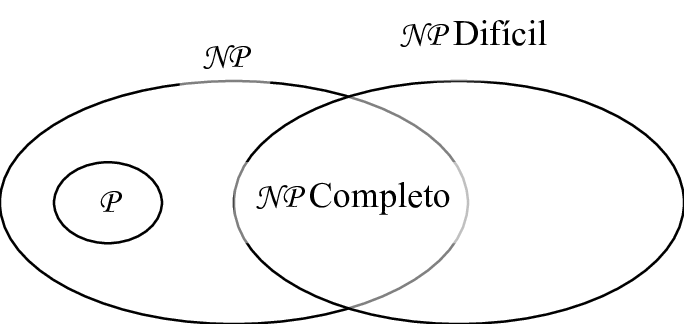
\includegraphics[width=0.5\textwidth]{img/relacaoDeConjuntos.png}
  \label{fig:complexidade}
  \\ \small Fonte: Adaptado de \citeonline{article}.
\end{figure}

\subsection{Algoritmos Fundamentais}
Para avaliar o impacto das linguagens no desempenho, foram selecionados algoritmos representativos das diferentes classes polinomiais, considerando tanto sua relevância teórica quanto aplicabilidade prática.

\subsubsection{Ordenação}
O algoritmo \eng{MergeSort} é representativo da classe P, com complexidade \(O(n \log n)\). Sua popularidade e ampla utilização tornam-no adequado como \eng{benchmark} para linguagens compiladas e interpretadas.

\subsubsection{Problemas de Otimização e Fatoração}
O Problema da Mochila (\eng{Knapsack}) foi escolhido por representar a classe NP-completo, desafiando linguagens em cenários de busca combinatória. Já a fatoração de inteiros (\eng{Factoring}), pertencente à classe NP, é relevante em aplicações como criptografia, permitindo analisar desempenho em problemas de verificação.

\subsubsection{Problemas Indecidíveis}
O Problema da Parada (\eng{Halting Problem}), embora indecidível em sua formulação geral, pode ser explorado em instâncias restritas, simulando programas com entradas controladas. Essa abordagem permite observar o comportamento das linguagens em termos de tempo de execução e uso de memória.

\subsection{Linguagens de Programação}
A linguagem de programação exerce impacto significativo na implementação de algoritmos, afetando diretamente tempo de execução, uso de memória e esforço de desenvolvimento.

\subsubsection{Critérios de Seleção}
As linguagens foram escolhidas com base em três critérios principais:
\begin{itemize}
  \item \textbf{Popularidade}: \eng{TIOBE Index} \citeonline{tiobe}, \eng{GitHub Octoverse} \citeonline{octoverse} e \eng{Stack Overflow Developer Survey} \citeonline{stackoverflow}.
  \item \textbf{Diversidade de paradigmas}: Compiladas (C, C++, Rust), interpretadas (Python, JavaScript) e híbridas (Java, C\#, Go, Kotlin, TypeScript).
  \item \textbf{Aplicabilidade acadêmica e industrial}: conforme \citeonline{sebesta2016}.
\end{itemize}

\subsubsection{Paradigmas e Modelos de Execução}
\begin{itemize}
  \item \textbf{Modelo de execução}: compilado ou interpretado.
  \item \textbf{Tipagem}: estática ou dinâmica.
  \item \textbf{Gerenciamento de memória}: manual ou automático.
\end{itemize}




\section{Materiais e Métodos}

Esta seção descreve o ambiente de experimentação e os procedimentos utilizados na condução dos testes comparativos. São apresentados os recursos de hardware e software empregados, as métricas consideradas na análise, os conjuntos de dados adotados e as etapas que compuseram o processo experimental. Essa organização visa garantir a reprodutibilidade do estudo e a clareza na interpretação dos resultados.

\subsection{Ambiente Experimental}
\begin{itemize}
  \item \textbf{Processador}: Intel Core i7-1165G7 (11ª geração), 2.80 GHz.
  \item \textbf{Memória RAM}: 16 GB DDR4 (2667 MHz).
  \item \textbf{Vídeo}: Intel Iris Xe Graphics.
  \item \textbf{SO}: Ubuntu 22.04 LTS.
\end{itemize}

\subsection{Métricas}
\begin{itemize}
  \item \textbf{Tempo de execução (\eng{Wall Clock})}: média de 30 execuções.
  \item \textbf{Uso de memória (RSS)}: pico residente (\texttt{/usr/bin/time}).
  \item \textbf{Complexidade de implementação}: \eng{SLOC} e complexidade ciclomática.
\end{itemize}

\subsection{Conjuntos de Dados}
\begin{itemize}
  \item \textbf{Pequeno}: \(n=10^3\)
  \item \textbf{Médio}: \(n=10^4\)
  \item \textbf{Grande}: \(n=10^5\)
\end{itemize}

\subsection{Procedimentos Experimentais}
\begin{enumerate}
  \item Implementação em todas as linguagens usando bibliotecas padrão.
  \item Compilação/execução com parâmetros padrão.
  \item 30 repetições por combinação linguagem $\times$ tamanho.
  \item Armazenamento e análise estatística (média e desvio-padrão).
\end{enumerate}



\section{Resultados}

\subsection{Tempo de Execução}
\begin{figure}[H]
  \caption{Figura 2 - Tempo médio de execução vs. tamanho do \eng{dataset} (geral, sem NP-completo).}
  \centering
  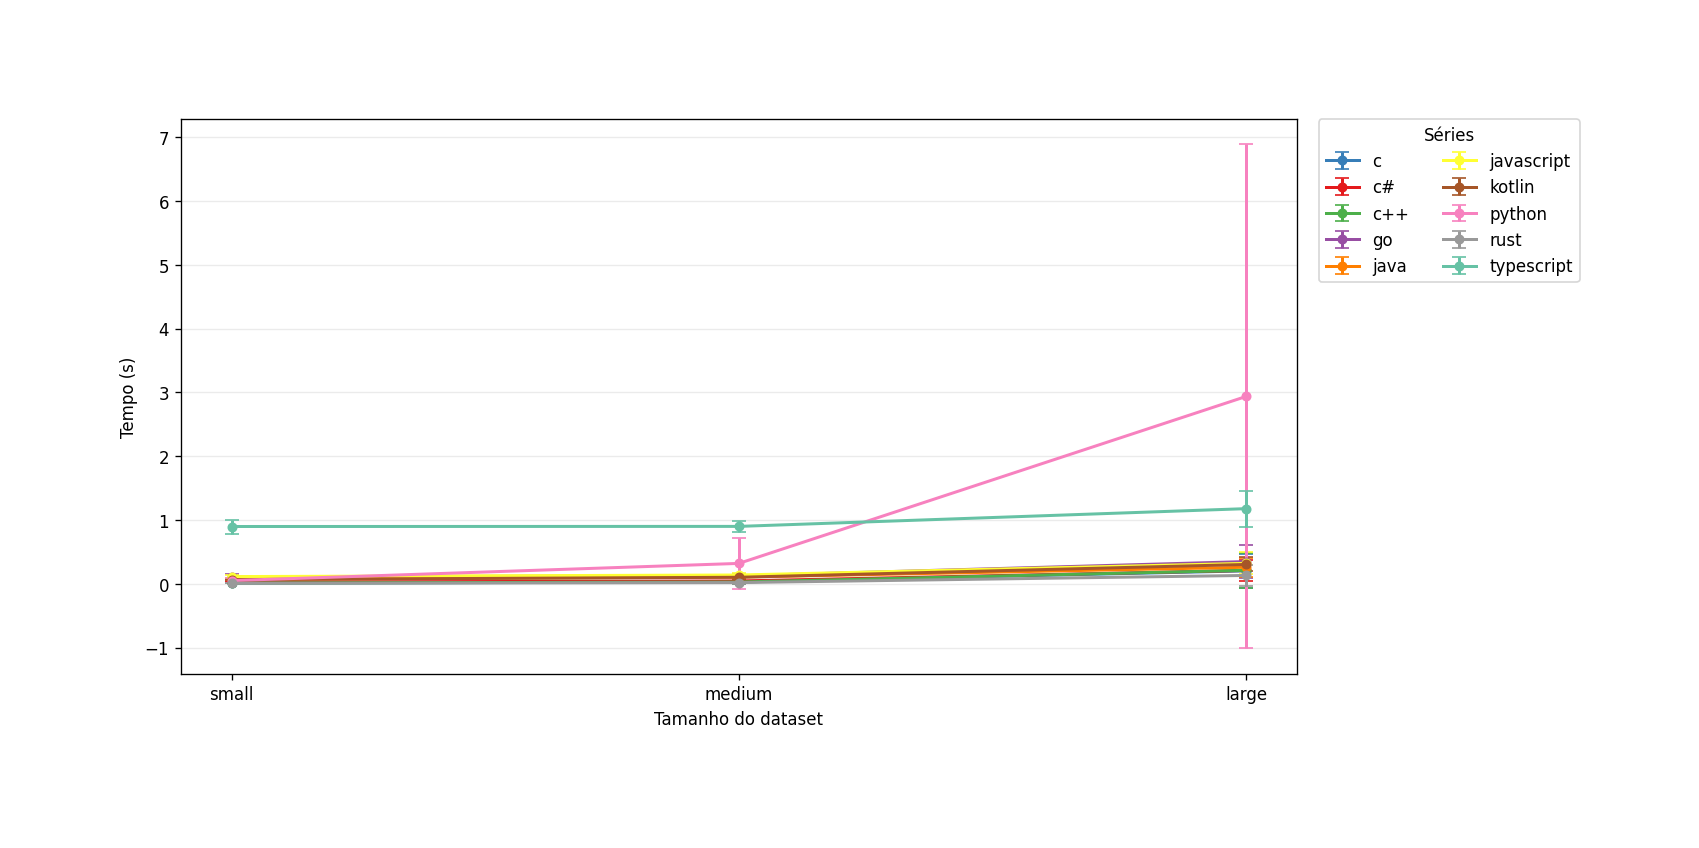
\includegraphics[width=0.8\textwidth]{img/tempo_vs_tamanho_all.png}
  \label{fig:tempo_execucao}
  \\ \small Fonte: Autor.
\end{figure}

\begin{table}[H]
  \caption{Tabela 1 - Tempo médio de execução (s) e desvio-padrão por linguagem e tamanho do \eng{dataset} (geral, sem NP-completo).}
  \centering
  \resizebox{\textwidth}{!}{%
  \begin{tabular}{l|cc|cc|cc|cc|cc|cc|cc|cc|cc|cc|cc|cc}
    \toprule
    \textbf{Tamanho} & \multicolumn{2}{c|}{\textbf{C}} & \multicolumn{2}{c|}{\textbf{C\#}} & \multicolumn{2}{c|}{\textbf{C++}} & \multicolumn{2}{c|}{\textbf{Go}} & \multicolumn{2}{c|}{\textbf{Java}} & \multicolumn{2}{c|}{\textbf{JS}} & \multicolumn{2}{c|}{\textbf{Kotlin}} & \multicolumn{2}{c|}{\textbf{Python}} & \multicolumn{2}{c|}{\textbf{Rust}} & \multicolumn{2}{c}{\textbf{TS}} \\
    \midrule
    & M & DP & M & DP & M & DP & M & DP & M & DP & M & DP & M & DP & M & DP & M & DP & M & DP \\
    \midrule
    \eng{small}  & 0.01 & 0.00 & 0.03 & 0.00 & 0.01 & 0.01 & 0.11 & 0.05 & 0.07 & 0.01 & 0.11 & 0.02 & 0.07 & 0.01 & 0.05 & 0.04 & 0.01 & 0.00 & 0.90 & 0.11 \\
    \eng{medium} & 0.03 & 0.03 & 0.04 & 0.02 & 0.03 & 0.03 & 0.12 & 0.03 & 0.10 & 0.02 & 0.14 & 0.03 & 0.10 & 0.01 & 0.32 & 0.40 & 0.02 & 0.02 & 0.90 & 0.09 \\
    \eng{large}  & 0.20 & 0.27 & 0.21 & 0.17 & 0.21 & 0.28 & 0.35 & 0.26 & 0.26 & 0.26 & 0.32 & 0.17 & 0.30 & 0.11 & 2.94 & 3.95 & 0.13 & 0.16 & 1.18 & 0.28 \\
    \bottomrule
  \end{tabular}%
  }
\end{table}

\subsection{Uso de CPU}
\begin{figure}[H]
  \caption{Figura 3 - Consumo máximo de CPU normalizada por tamanho.}
  \centering
  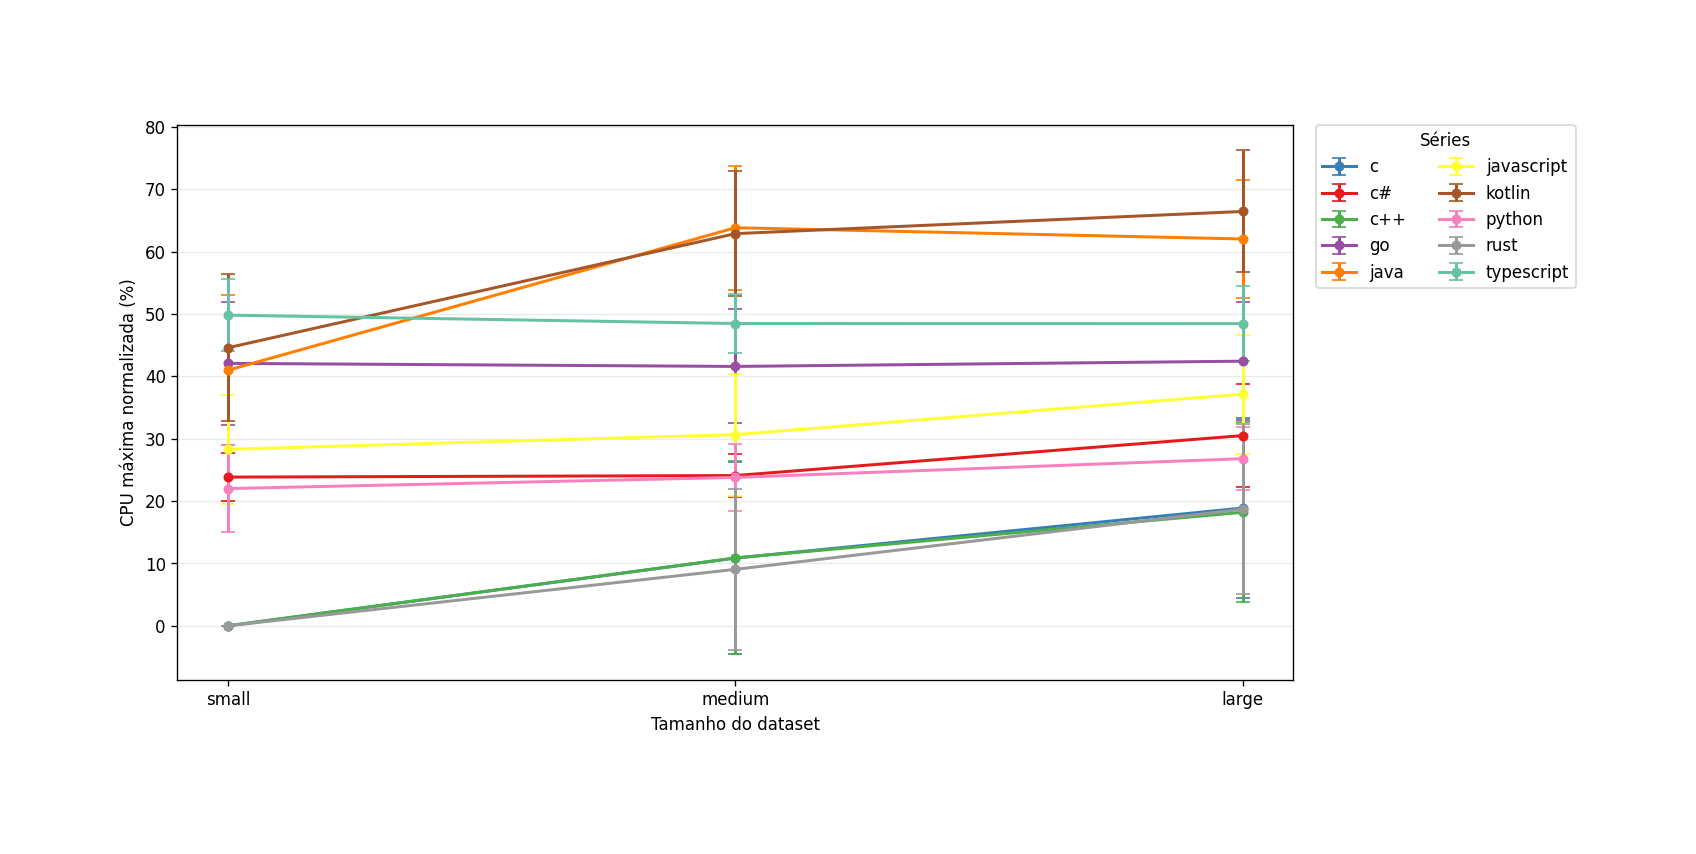
\includegraphics[width=0.8\textwidth]{img/cpu_vs_tamanho_all.png}
  \label{fig:cpu}
  \\ \small Fonte: Autor.
\end{figure}

\begin{table}[H]
  \caption{Tabela 2 - Consumo máximo de CPU normalizada (\%) por linguagem e tamanho de \eng{dataset}.}
  \centering
  \resizebox{\textwidth}{!}{%
  \begin{tabular}{l|cc|cc|cc|cc|cc|cc|cc|cc|cc|cc|cc|cc}
    \toprule
    \textbf{Tamanho} & \multicolumn{2}{c|}{\textbf{C}} & \multicolumn{2}{c|}{\textbf{C\#}} & \multicolumn{2}{c|}{\textbf{C++}} & \multicolumn{2}{c|}{\textbf{Go}} & \multicolumn{2}{c|}{\textbf{Java}} & \multicolumn{2}{c|}{\textbf{JS}} & \multicolumn{2}{c|}{\textbf{Kotlin}} & \multicolumn{2}{c|}{\textbf{Py}} & \multicolumn{2}{c|}{\textbf{Rust}} & \multicolumn{2}{c}{\textbf{TS}} \\
    \midrule
    & M & DP & M & DP & M & DP & M & DP & M & DP & M & DP & M & DP & M & DP & M & DP & M & DP \\
    \midrule
    \eng{small}  & 0.00 & 0.00 & 23.84 & 3.86 & 0.00 & 0.00 & 42.08 & 9.85 & 40.99 & 12.08 & 28.30 & 8.78 & 44.59 & 11.82 & 22.00 & 7.01 & 0.00 & 0.00 & 49.82 & 5.72 \\
    \eng{medium} & 10.86 & 15.46 & 24.09 & 3.43 & 10.88 & 15.48 & 41.59 & 9.14 & 63.83 & 9.91 & 30.66 & 9.79 & 62.89 & 10.08 & 23.79 & 5.35 & 9.05 & 12.91 & 48.47 & 4.76 \\
    \eng{large}  & 18.88 & 14.40 & 30.50 & 8.21 & 18.21 & 14.42 & 42.43 & 9.46 & 62.03 & 9.42 & 37.15 & 9.55 & 66.44 & 9.78 & 26.79 & 5.04 & 18.70 & 13.65 & 48.45 & 6.07 \\
    \bottomrule
  \end{tabular}%
  }
\end{table}

\subsection{Uso de Memória}
\begin{figure}[H]
  \caption{Figura 4 - Uso máximo de memória vs. tamanho do \eng{dataset}.}
  \centering
  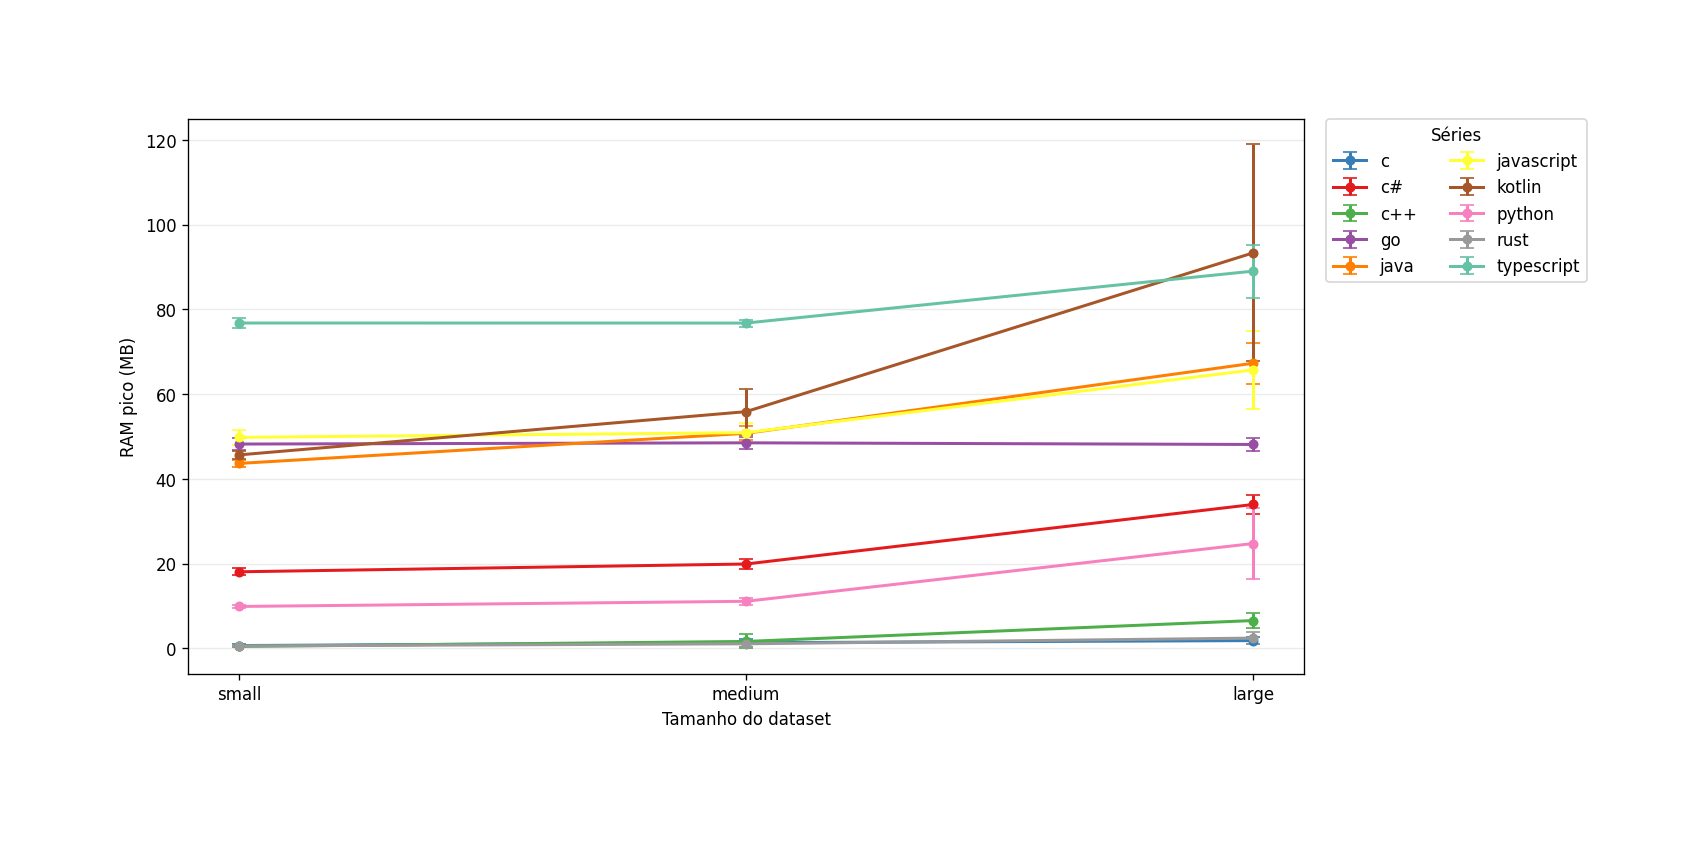
\includegraphics[width=0.8\textwidth]{img/ram_vs_tamanho_all.png}
  \label{fig:memoria}
  \\ \small Fonte: Autor.
\end{figure}

\begin{table}[H]
  \caption{Tabela 3 - Uso máximo de memória (MB) e desvio padrão (DP).}
  \centering
  \resizebox{\textwidth}{!}{%
  \begin{tabular}{l|cc|cc|cc|cc|cc|cc|cc|cc|cc|cc|cc|cc}
    \toprule
    \textbf{Tamanho} & \multicolumn{2}{c|}{\textbf{C}} & \multicolumn{2}{c|}{\textbf{C\#}} & \multicolumn{2}{c|}{\textbf{C++}} & \multicolumn{2}{c|}{\textbf{Go}} & \multicolumn{2}{c|}{\textbf{Java}} & \multicolumn{2}{c|}{\textbf{JS}} & \multicolumn{2}{c|}{\textbf{Kotlin}} & \multicolumn{2}{c|}{\textbf{Py}} & \multicolumn{2}{c|}{\textbf{Rust}} & \multicolumn{2}{c}{\textbf{TS}} \\
    \midrule
    & M & DP & M & DP & M & DP & M & DP & M & DP & M & DP & M & DP & M & DP & M & DP & M & DP \\
    \midrule
    \eng{small}  & 0.68 & 0.29 & 18.08 & 0.81 & 0.48 & 0.06 & 48.23 & 1.51 & 43.65 & 0.80 & 49.80 & 1.70 & 45.66 & 0.87 & 9.90 & 0.41 & 0.58 & 0.30 & 76.78 & 1.29 \\
    \eng{medium} & 1.35 & 0.94 & 19.92 & 1.25 & 1.65 & 1.66 & 48.52 & 1.46 & 50.76 & 1.62 & 50.92 & 2.22 & 55.87 & 5.43 & 11.12 & 0.79 & 1.09 & 0.75 & 76.78 & 0.82 \\
    \eng{large}  & 1.85 & 0.86 & 33.97 & 2.18 & 6.58 & 1.86 & 48.13 & 1.49 & 67.30 & 4.80 & 65.73 & 9.21 & 93.35 & 25.56 & 24.76 & 8.39 & 2.44 & 1.46 & 89.03 & 6.27 \\
    \bottomrule
  \end{tabular}%
  }
\end{table}

\subsection{Qualidade da Solução da Heurística}
\begin{figure}[H]
  \caption{Figura 5 - Exato vs. heurístico (NP-completo) em tempo de execução.}
  \centering
  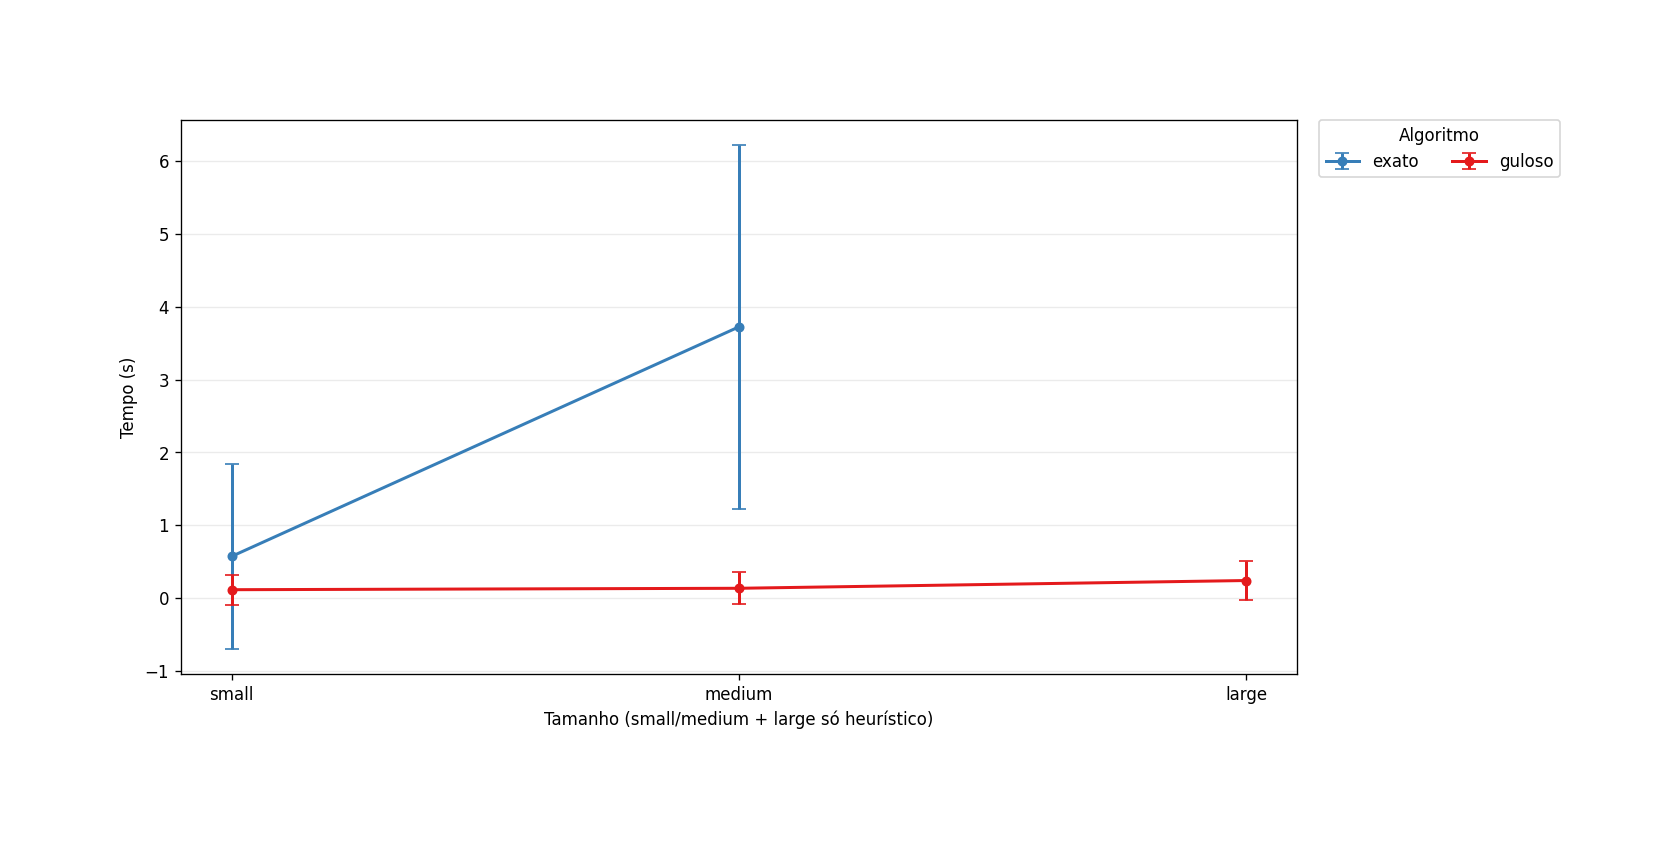
\includegraphics[width=0.8\textwidth]{img/qualidade_heuristica.png}
  \label{fig:qualidade}
  \\ \small Fonte: Autor.
\end{figure}

\begin{table}[H]
  \caption{Tabela 4 - Comparação de tempo de execução entre solução exata e heurística (NP-completo).}
  \centering
  \resizebox{0.8\textwidth}{!}{%
  \begin{tabular}{c|cc|cc}
    \toprule
    \textbf{Tamanho} & \multicolumn{2}{c|}{\textbf{Exato}} & \multicolumn{2}{c}{\textbf{Heurístico (Guloso)}} \\
    \midrule
    & M (s) & DP (s) & M (s) & DP (s) \\
    \midrule
    \eng{small}  & 0.57 & 1.27 & 0.11 & 0.21 \\
    \eng{medium} & 3.72 & 2.50 & 0.13 & 0.22 \\
    \eng{large}  & -- & -- & 0.24 & 0.26 \\
    \bottomrule
  \end{tabular}%
  }
\end{table}

\subsection{Linhas de Código}
\begin{figure}[H]
  \caption{Figura 6 - \eng{SLOC} por linguagem e algoritmo.}
  \centering
  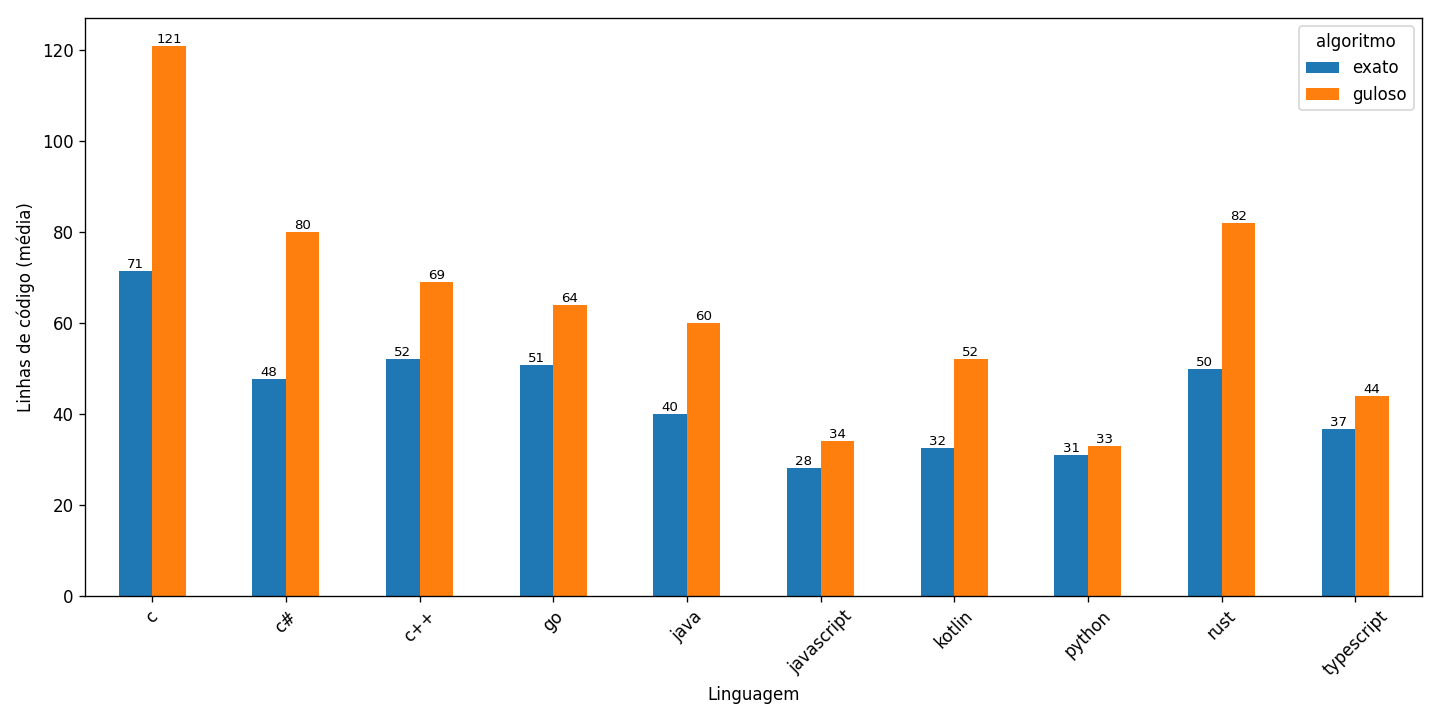
\includegraphics[width=0.8\textwidth]{img/linhas_codigo_linguagem_algoritmo.png}
  \label{fig:sloc}
  \\ \small Fonte: Autor.
\end{figure}

\section{Conclusão}
Este trabalho apresentou uma análise comparativa de algoritmos implementados em diferentes linguagens de programação, com foco em métricas de desempenho (tempo de execução, uso de CPU e memória) e complexidade de implementação (\eng{SLOC}). O objetivo central foi investigar o impacto da linguagem de programação na eficiência computacional, considerando cenários controlados e instâncias de diferentes tamanhos.

Os resultados evidenciaram que linguagens compiladas de baixo nível, como C, C++ e Rust, mantiveram desempenho superior em termos de tempo e memória, confirmando sua adequação a aplicações que demandam alta eficiência. Em contrapartida, linguagens interpretadas como Python, JavaScript e TypeScript, embora apresentem menor desempenho em grandes volumes de dados, destacaram-se pela simplicidade de implementação e expressividade. Linguagens intermediárias, como Java, Kotlin e Go, mostram-se adequadas para sistemas distribuídos e aplicações de larga escala, em que o equilíbrio entre desempenho e portabilidade é determinante.

A análise da heurística aplicada ao problema NP-completo demonstrou que abordagens aproximadas oferecem soluções próximas ao ótimo em frações do tempo exigido pelo algoritmo exato, viabilizando aplicações práticas em cenários de maior escala. Esse achado reforça o \eng{trade-off} entre precisão e eficiência computacional, fundamental em problemas de alta complexidade.

Como limitações, destaca-se a utilização de um único ambiente experimental, o que restringe a generalização dos resultados para diferentes arquiteturas de hardware e sistemas operacionais. Ademais, foram considerados apenas algoritmos representativos das classes P, NP, NP-completo e NP-difícil, não abrangendo a totalidade do espectro de problemas computacionais.

Como perspectivas futuras, propõe-se ampliar os experimentos para incluir diferentes configurações de hardware, explorar métricas adicionais como consumo energético e escalabilidade em ambientes distribuídos, além de avaliar outras linguagens emergentes e paradigmas de programação. Tais investigações podem aprofundar a compreensão dos impactos da linguagem de programação no desempenho e orientar decisões ainda mais embasadas em contextos acadêmicos e industriais.

% ------------------
% Referências
% ------------------
\renewcommand{\refname}{REFERÊNCIAS}
\begingroup
\setstretch{1.0}
\bibliographystyle{abntex2-alf}
\bibliography{Bibliografia}
\endgroup

\end{document}
